\documentclass[a4paper,12pt]{article}
%\usepackage{latexsym}
%\usepackage[MeX]{polski}
%\usepackage[latin2]{inputenc}% ew. utf8 lub cp1250
\usepackage{enumitem}
%\usepackage{nopageno}
\usepackage{geometry}
\usepackage{graphicx}
\usepackage{wrapfig}
\usepackage{xcolor}
\usepackage[square,sort&compress,comma,numbers]{natbib}
\usepackage{iopams}
\usepackage{amsmath}
\usepackage[ruled,vlined]{algorithm2e}
\newgeometry{tmargin=1.5cm, bmargin=1.5cm, lmargin=2.5cm, rmargin=2.5cm}
\newcommand{\rmd}{\mathrm{d}}
\bibliographystyle{sms}
% Zdefiniowanie autora i~tytułu:
\author{Piotr Fiborek}
%\date{}
\title{Numerical analysis of Guided Waves propagation in Honeycomb Sandwich Composites\\
(\textit{Analiza numeryczna propagacji fal prowadzonych w wielowarstwowych materia\l{}ach przek\l{}adkowych z rdzeniem o strukturze plastra miodu})}
\begin{document}
\maketitle
\thispagestyle{empty}
\section{Introduction}
\label{sec:intro}
Honeycomb Sandwich Composite~(HSC) is a type of multi-layered structure, which 
is composed of the mid-core with the geometry of honeycomb sandwiched between 
thin skins.
They are widely used in the aerospace, marine and automotive industries due to 
the high strength-to-weight ratio, high energy absorption capability and 
effective acoustic insulation. However, these complex structures are exposed to 
a risk of different types of failures, e.g. hidden disbonds between the skin 
and the core.



The most common numerical modelling of the phenomenon of GW in CHSP found in 
the literature is a calculation of the effective material properties of the 
honeycomb structure by the homogenisation process~\cite{qi2008ultrasonic, 
mustapha2011assessment, baid2015dispersion, sikdar2016guided}.
However, this method is not able to adequately present the phenomenon of 
propagation of elastic waves in such material.
A more accurate model will be achieved if the real geometry of the hexagonal 
cell is retained.
Ruzzenne et al. conducted a parametric study through the finite element model 
of the unit cell and the application of the theory of periodic structures 
\cite{ruzzene2003wave}.
Recently, the simulations of the wave propagation in HSC have been conducted 
with the commercially available finite element code~\cite{song2009guided, 
hosseini2013numerical, tian2015wavenumber, zhao2018wave}.
However, finite element simulations (FEM) of GW are inefficient as they require 
significant amounts of memory and are time-consuming.

This paper presents a new model of propagating GW in HSC using the time-domain 
spectral element method (SEM).
The SEM was originally developed for the numerical solution of the fluid flow 
in a channel by Patera~\cite{patera1984spectral} but has also been successfully 
implemented for elastic wave propagation~\cite{ostachowicz2011guided}.
SEM combines the flexibility of the FEM and accuracy of the techniques based on 
Fourier transform. 

In order to reduce a global number of degree of freedom (DOF) in the 
simulation, skins, adhesive layers and each wall composing a hexagonal cell of 
the core are modelled by two-dimensional (2D) spectral elements.
The displacements of the cell are calculated in the local coordinate system, 
and then, through the transformation matrix, they are transformed into the 
global coordinate system. Subsequently, the core is connected to the skin 
plates so that displacements of common geometrical points of both elements are 
the same in each direction of the main axes.
This type of connection is implemented by means of interface elements based on 
Lagrange multipliers, which are interpreted as forces responsible for 
determining the appropriate displacements of nodes.
By using the interface, it is possible to model skin plates with 2D elements.
This type of approach will reduce the number of degrees of freedom, which in 
turn will shorten the calculation time and reduce the need for operational 
memory.

Wave excitation was realised by the piezoelectric (PZT) transducer, which was 
modelled by a three-dimensional (3D) spectral element with the 
electromechanical coupling.
\section{The time-domain spectral element method formulation}
\label{sec:time_SEM}
\subsection{The spectral element method}
\label{sec:sem}
The idea of the SEM is similar to the FEM.
Both methods use a division of the modelled domain into finite elements.
Also, imposition of the arbitrary boundary conditions and external forces in 
particular nodes is similar.
The main difference between those methods is a distribution of nodes in 
elements and approximation function describing changes of displacements.
The element nodes in SEM are non-uniformly distributed, and they are obtained 
as the roots of Eq.~(\ref{eq:nodes}).

\begin{eqnarray}
(1-\xi^2)P'_{p-1}(\xi)=0,\ (1-\eta^2)P'_{q-1}(\eta)=0,\ (1-\zeta^2)P'_{r-1}(\zeta)=0
	\label{eq:nodes}
\end{eqnarray} 
where $\xi,\eta,\zeta\in[-1,1]$, $P_{p-1},P_{q-1}$ and $P_{r-1}$ are Legendre polynomials of degree (p-1), (q-1) and (r-1), respectively and symbol $'$ denotes the first derivative. 3D shape functions are constructed as a tensor product of the 1D shape functions $\textbf{N}_m(\xi)$, $\textbf{N}_n(\eta)$ and $\textbf{N}_l(\zeta)$ defined by the Lagrange interpolating polynomials of order $p-1$, $q-1$ and $r-1$, respectively.

The element matrices are obtained according to Gauss-Lobatto-Legrendre (GLL) integration scheme where the integration points coincide with the element nodes and associated weights ${w}_m$, ${w}_n$ and ${w}_l$ are computed as:
\begin{eqnarray}
{w}_m &=& \frac{2}{p(p-1)(P_{p-1}(\xi_m))^2},\nonumber\\
{w}_n &=& \frac{2}{q(q-1)(P_{q-1}(\eta_n))^2},\nonumber \\
{w}_l &=& \frac{2}{r(r-1)(P_{r-1}(\zeta_l))^2},
\label{eq:weights}
\end{eqnarray}
Due to utilised GLL integration scheme and the orthogonality of shape functions obtained mass matrix is diagonal.
\subsection{2D spectral element formulation}
\label{sec:2D_SEM}
2D spectral elements are formulated according to the first-order shear 
deformation theory~\cite{reissner1945effect, mindlin1951influence} so that 
three displacement components \textbf{u}, \textbf{v} and \textbf{w}, can be 
expressed as:
\begin{eqnarray}
\left [ \begin{array}{c}
\textbf{u}^e(\xi,\eta,\zeta) \\
\textbf{v}^e(\xi,\eta,\zeta) \\
\textbf{w}^e(\xi,\eta,\zeta)
\end{array} \right] = 
\left [ \begin{array}{c}
\textbf{u}_0^e(\xi,\eta) + z\boldsymbol{\varphi}_x^e(\xi,\eta)\\
\textbf{v}_0^e(\xi,\eta) + z\boldsymbol{\varphi}_y^e(\xi,\eta)\\
\textbf{w}_0^e(\xi,\eta) \\
\end{array} \right]
\end{eqnarray}
where $\textbf{u}_0^e$, $\textbf{v}_0^e$ and $\textbf{w}_0^e$ denote the 
displacements of a point on the mid-plane, $\boldsymbol{\varphi}_x^e$, 
$\boldsymbol{\varphi}_y^e$ are the rotations of the normal to the mid-plane 
with respect to axes \textit{x} and \textit{y}, respectively.
\begin{eqnarray}
\left [ \begin{array}{c}
\textbf{u}_0^e(\xi,\eta) \\
\textbf{v}_0^e(\xi,\eta) \\
\textbf{w}_0^e(\xi,\eta) \\
\boldsymbol{\varphi}_x^e(\xi,\eta) \\
\boldsymbol{\varphi}_y^e(\xi,\eta)
\end{array} \right]
& = & \textbf{N}^e(\xi,\eta)\widehat{\textbf{d}}^e\nonumber\\
& = & \sum_{n=1}^q\sum_{m=1}^p\textbf{N}_m^e(\xi)\textbf{N}_n^e(\eta)
\left [ \begin{array}{c}
\widehat{\textbf{u}}_0^e \\
\widehat{\textbf{v}}_0^e \\
\widehat{\textbf{w}}_0^e \\
\widehat{\boldsymbol{\varphi}}_x^e \\
\widehat{\boldsymbol{\varphi}}_y^e
\end{array} \right]
\end{eqnarray}
The bending strain components can be written as~\cite{ferreira2008matlab}:
\begin{eqnarray}
\bepsilon_b^e(\xi,\eta)=\textbf{B}_b^e\widehat{\textbf{d}}^e
\end{eqnarray}
where $\textbf{B}_b^e$ is curvature-displacement matrix calculated as:
\begin{eqnarray}
\textbf{B}_b^e=\textbf{L}_b\textbf{N}^e(\xi,\eta)
\end{eqnarray}
\begin{eqnarray}
	\textbf{L}_b=\left [
	\begin{array}{ccccc}
		\frac{\partial }{\partial x} & 0 & 0 & 0 & 0\\
		0 & \frac{\partial }{\partial y} & 0 & 0 & 0\\
		\frac{\partial }{\partial y} & \frac{\partial }{\partial x} & 0 & 0 & 0\\
		0 & 0 & 0 & -\frac{\partial }{\partial x} & 0\\
		0 & 0 & 0 & 0 & -\frac{\partial }{\partial y}\\
		0 & 0 & 0 & -\frac{\partial }{\partial y} & -\frac{\partial }{\partial x}
	\end{array} \right],\ \\
  \left [
	\begin{array}{c}
		\frac{\partial }{\partial x}\\
		\frac{\partial }{\partial y}
	\end{array} \right] =\textbf{J}^{-1}
	\left [
	\begin{array}{c}
		\frac{\partial }{\partial \xi}\\
		\frac{\partial }{\partial \eta}
	\end{array} \right], \ 
	\textbf{J}=\left [
	\begin{array}{cc}
		\partial_\xi x & {\partial_\xi y} \\
		\partial_\eta x & {\partial_\eta y}
	\end{array} \right] \nonumber
\end{eqnarray}
The shear strain components can be written as~\cite{ferreira2008matlab}:
\begin{eqnarray}
\bepsilon_s^e(\xi,\eta)=\textbf{B}_s^e\widehat{\textbf{d}}^e
\end{eqnarray}
where $\textbf{B}_s^e$ is curvature-displacement matrix calculated as:
\begin{eqnarray}
\textbf{B}_s^e=\textbf{L}_s\textbf{N}^e(\xi,\eta)
\end{eqnarray}
\begin{eqnarray}
\textbf{L}_s=\left [
\begin{array}{ccccc}
0 & 0 & \frac{\partial }{\partial x} & -1 & 0 \\
0 & 0 & \frac{\partial }{\partial y} & 0 & -1
\end{array} \right]
\end{eqnarray}
\subsection{3D model of the PZT transducer}
\label{sec:3D_SEM}
The displacements of the PZT transducer are defined by three displacement components \textbf{u}, \textbf{v} and \textbf{w}, and can be express in a form:
\begin{eqnarray}
\left [ \begin{array}{c}
\textbf{u}^e(\xi,\eta,\zeta) \\
\textbf{v}^e(\xi,\eta,\zeta) \\
\textbf{w}^e(\xi,\eta,\zeta)
\end{array} \right]
& = & \textbf{N}^e(\xi,\eta, \zeta)\widehat{\textbf{d}}^e\nonumber\\
& = & \sum_{l=1}^r\sum_{n=1}^q\sum_{m=1}^p\textbf{N}_m^e(\xi)\textbf{N}_n^e(\eta)\textbf{N}_l^e(\zeta)
\left [ \begin{array}{c}
\widehat{\textbf{u}}^e(\xi_m,\eta_n,\zeta_l) \\
\widehat{\textbf{v}}^e(\xi_m,\eta_n,\zeta_l) \\
\widehat{\textbf{w}}^e(\xi_m,\eta_n,\zeta_l)
\end{array} \right]
\label{eq:3D_displ}
\end{eqnarray}
where $\widehat{\textbf{u}}^e$, $\widehat{\textbf{v}}^e$ and $\widehat{\textbf{w}}^e$ are nodal values.
Six components of the strain matrix are approximated as follow 
\cite{kudela20093d}:
\begin{eqnarray}
\bepsilon^e(\xi,\eta,\zeta)=\textbf{B}_{d}^e\widehat{\textbf{d}}^e
\end{eqnarray}
where $\textbf{B}_{d}^e$ is strain-nodal displacement matrix calculated as:
\begin{eqnarray}
\textbf{B}_{d}^e=\textbf{L}\textbf{N}^e(\xi,\eta,\zeta)
\end{eqnarray}
\begin{eqnarray}
\textbf{L}=\left [
\begin{array}{ccc}
\frac{\partial }{\partial x} & 0 & 0\\
0 & \frac{\partial }{\partial y} & 0\\
0 & 0 & \frac{\partial }{\partial z}\\
0 & \frac{\partial }{\partial z} & \frac{\partial }{\partial y}\\
\frac{\partial }{\partial z} & 0 & \frac{\partial }{\partial x}\\
\frac{\partial }{\partial y} & \frac{\partial }{\partial x} & 0
\end{array} \right],\ 
\left [
\begin{array}{c}
\frac{\partial }{\partial x}\\
\frac{\partial }{\partial y}\\
\frac{\partial }{\partial z}
\end{array} \right] =\textbf{J}^{-1}
\left [
\begin{array}{c}
\frac{\partial }{\partial \xi}\\
\frac{\partial }{\partial \eta}\\
\frac{\partial }{\partial \zeta}
\end{array} \right], \ 
\textbf{J}=\left [
\begin{array}{ccc}
\partial_\xi x & {\partial_\xi y} & {\partial_\xi z}\\
\partial_\eta x & {\partial_\eta y} & {\partial_\eta z}\\
\partial_\zeta x & {\partial_\zeta y} & {\partial_\zeta z}
\end{array} \right]
\end{eqnarray}

The electromechanical coupling is governed by the linear constitutive equation 
of piezoelectric material according to~\cite{giurgiutiumicromechatronics} and 
it is expressed by:
\begin{eqnarray}
\left [ 
\begin {array}{c}
\bsigma\\
\textbf{D}
 \end{array}\right ]=
\left [ 
\begin{array}{cc}
\textbf{c}^E & -\textbf{e}^T \\
\textbf{e} & \bepsilon^S 
\end{array} \right ]
\left[ 
\begin{array}{c}
\textbf{S}\\
\textbf{E} 
\end{array} \right ]
\end{eqnarray}
where \textbf{c}$^E$, \textbf{e} and $\bepsilon^S$ are tensors of elastic, 
piezoelectric and dielectric constants, respectively, \textbf{E} and \textbf{D} 
are the electric field and electric displacement, $\bsigma$ and \textbf{S} are 
stress and strain.
The superscripts E and S indicate that quantities are measured at zero electric 
fields and zero strain, respectively and the subscript T denotes transpose 
matrix.
Electric field vector can be expressed as:
\begin{eqnarray}
\textbf{E}^e=-\textbf{B}_\phi^e \widehat{\bphi}^e
\end{eqnarray}
where \textbf{B}$_\phi^e$ is electric-nodal potential matrix calculated as:
\begin{eqnarray}
\textbf{B}_\phi^e=
\left[ \begin{array}{c}
\frac{\partial }{\partial \xi}\\
\frac{\partial }{\partial \eta}\\
\frac{\partial }{\partial \zeta}
\end{array} \right]\textbf{N}^e(\xi,\eta,\zeta)
\end{eqnarray}

\subsection{Displacements coupling at the substructures interface}
\label{sec:interface}
The present model of the sandwich panel consists of 2D and 3D elements. 
Moreover, there are non-matching grids between two adjacent substructures. 
These involve connecting them by imposing the compatibility of the 
displacements at the interface, see Fig.~\ref{fig:interface}. The coupling can 
be expressed as:
\begin{eqnarray}
\left\{\begin{array}{c}
	\textbf{u}\\
	\textbf{v}\\
	\textbf{w}
	\end{array}\right\}_{s_{i1}}^{\Gamma^i}-
	\left\{\begin{array}{c}
	\textbf{u}\\
	\textbf{v}\\
	\textbf{w}
	\end{array}\right\}_{s_{i2}}^{\Gamma^i}=
	\left\{\begin{array}{c}
	\textbf{0}\\
	\textbf{0}\\
	\textbf{0}
	\end{array}\right\}
\label{eq:coupling}
\end{eqnarray}
\begin{figure}
	\begin{center}
		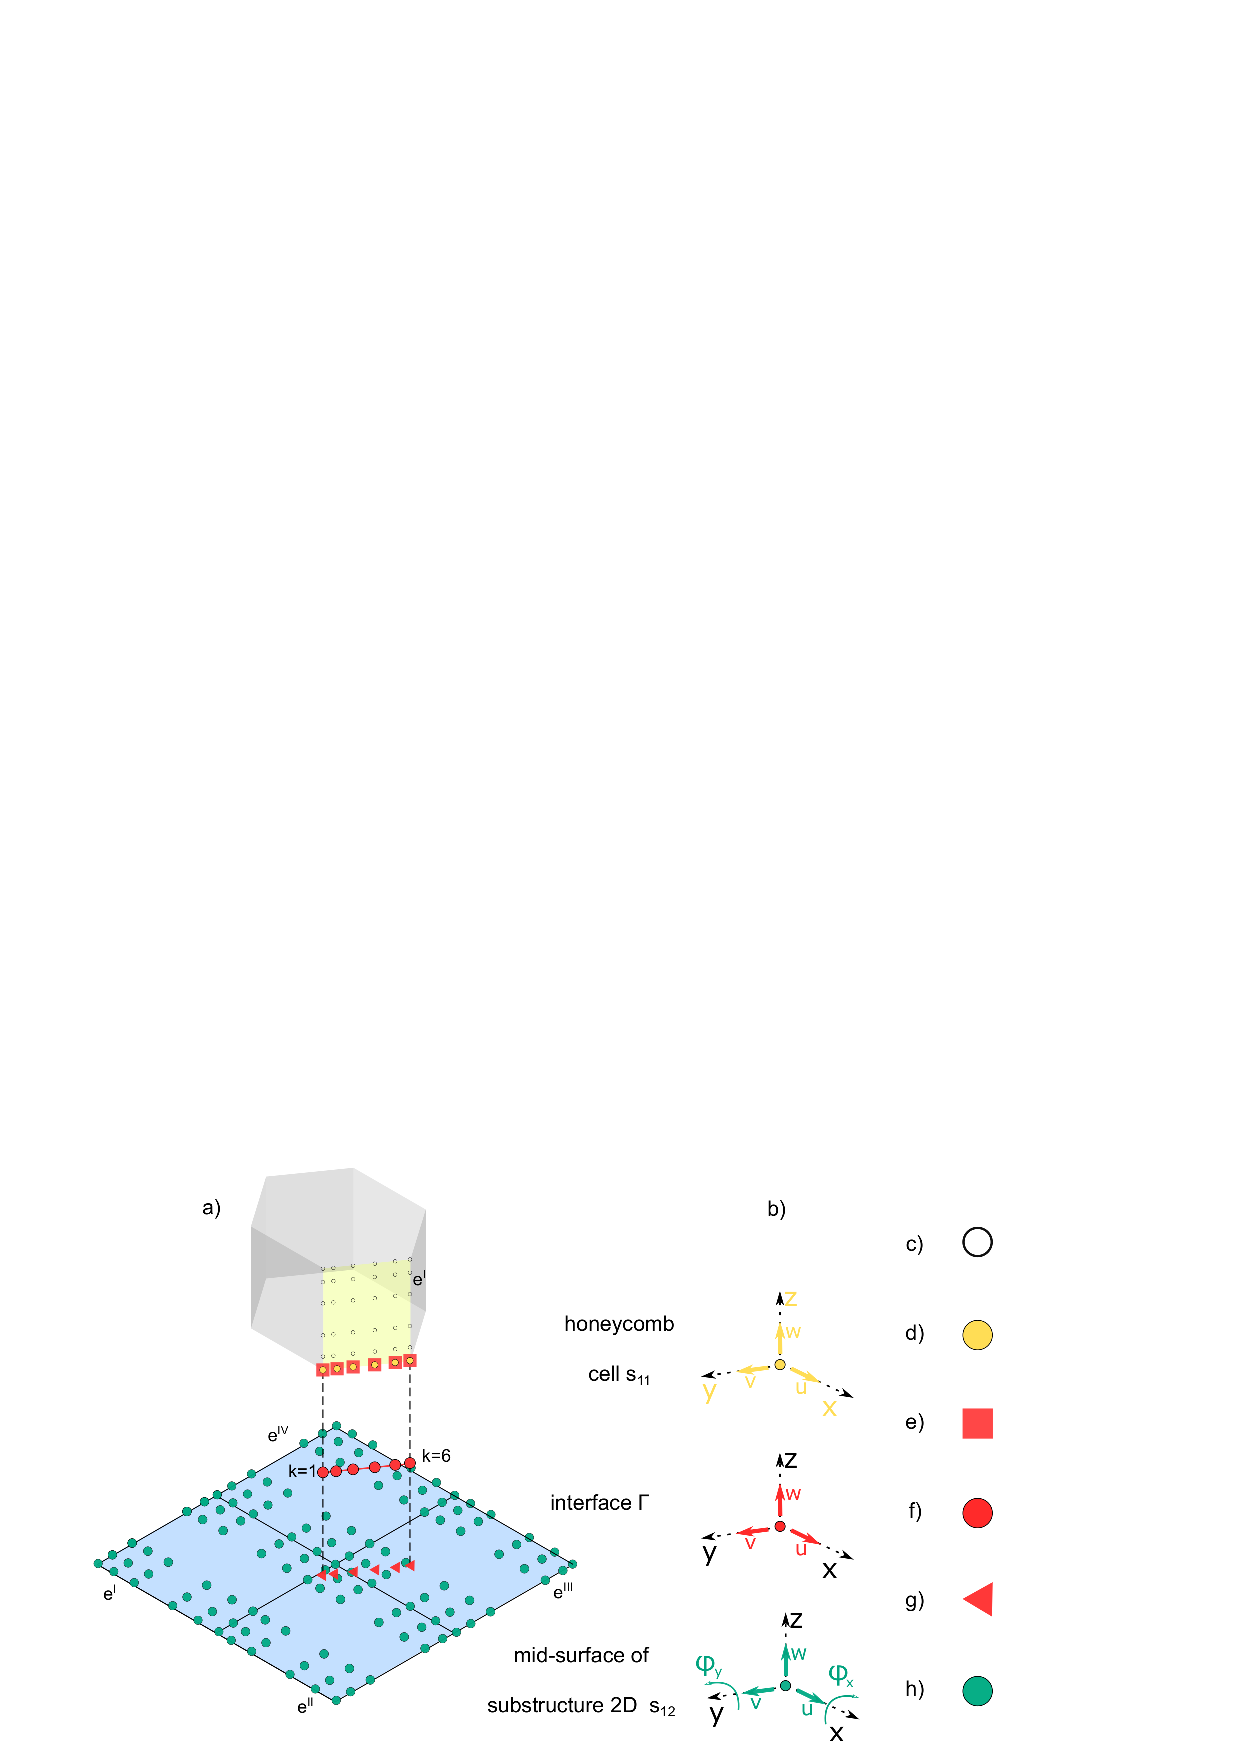
\includegraphics[width=1\linewidth]{../../../figures/png/interface_honeycomb.png}
	\end{center}
	\caption{Interface setup: a) interface coupling, b) the substructures and 
	the interface degree of freedom, c) all the nodes of honeycomb wall except 
	bottom layer nodes, d) the nodes of the 3D substructure at the bottom 
	layer, e) the interface nodes projected to the bottom layer of the 3D 
	substructure, f) the interface nodes, g) the interface nodes projected to 
	mid-surface of the 2D substructure, h) the nodes of the 2D substructure}
	\label{fig:interface}
\end{figure}
For the whole structure, equation~\ref{eq:coupling} can be written in the 
matrix form:
\begin{eqnarray}
\textbf{G}\textbf{d}=\textbf{0}
\label{eq:cond_disp}
\end{eqnarray}
where \textbf{G} is the coupling matrix which contains the equations to interpolate the substructures displacements at the interfaces, and $\textbf{d}$ is a global vector of displacements for $nS$ number of substructures, composed as:
\begin{eqnarray}
\textbf{d} = \left\{\begin{array}{cccc}
\textbf{d}_1, & \textbf{d}_2, &\ldots, & \textbf{d}_{nS}
\end{array}\right\}^T
\label{eq:displacements}
\end{eqnarray}

General formulation of the matrix \textbf{G} is proposed in Algorithm 
\ref{alg:G_matrix}.
The main task of the algorithm is to calculate shape functions for each 
adjacent substructures at the points $X_p=(x_p^k,y_p^k)$, which are projections 
of the interface nodes onto these substructures.
The shape function can be calculated after finding an owner element and local 
coordinates of the points. Owner element is a spectral element in domain of the 
substructure $s_{ij}$ which contains interface node, for example interface node 
$k=6$ (see Fig.~\ref{fig:interface}a)) is located in element $e^I$ and 
$e^{III}$ for the substructures $s_{i1}$ and $s_{i2}$, respectively.
It can be found within two ways: using Matlab's built-in function 
\verb+inpolygon+ or more efficient procedure proposed by Silva et al. 
\cite{silva2009exact} which was used in the current implementation.
The transformation from global to local coordinates was realized by the 
iterative method presented in the work of Li et al.~\cite{li2014efficient}.

\begin{algorithm}[H]
	\SetAlgoLined
	\KwResult{coupling matrix \textbf{G}}
	create empty $nI \times nS$ cell array: $\mathbf{G} = cell(nI,nS)$\;
	\For{i = 1 \KwTo nI}{
		find two common structures of interface $\Gamma^i$: $s_i = (s_{i1},s_{i2})$\;
		\For{j = 1 \KwTo 2}{
			create $n^{\Gamma^i}\times n^{s_{ij}}$ null matrix $\mathbf{G}^{s_{ij}}_i$,\\
			\For{k = 1 \KwTo $n^{\Gamma^i}$} {
				find $ownerElement^{s_{ij}}_k$ in the structure $s_{ij}$ containg interface node $k$ with global coordinates vector: $X_p=(x^k_p,y^k_p)$\;
				assign vector $X_e=(x_e,y_e)$ of coordinates of all nodes in $ownerElement^{s_{ij}}_k$\;
				assign initial coordinates $X_{\kappa}=(x^k_{\kappa},y^k_{\kappa})$ to the nearest node in $ownerElement^{s_{ij}}_k$ to node $k$\;
				transform global coordinates $X_{\kappa}$ to local coordinate system $\xi_{\kappa}=\xi(X_{\kappa});\quad \eta_{\kappa}=\eta(X_{\kappa})$\;
				\While{$\left|X_p-X_{\kappa}\right|>tol$}{
					$\xi_{\kappa+1}=\xi_{\kappa}+(J^{-1}_{\kappa})_{11}.*(x^k_p-x_{\kappa}^k)+(J^{-1}_{\kappa})_{12}.*(y^k_p-y_{\kappa}^k)$\;
					$\eta_{\kappa+1}=\eta_{\kappa}+(J^{-1}_{\kappa})_{21}.*(x^k_p-x_{\kappa}^k)+(J^{-1}_{\kappa})_{22}.*(y^k_p-y_{\kappa}^k)$\;
					$X_{\kappa}=N(\xi_{\kappa+1},\eta_{\kappa+1})X_e$\;
				}
				$\xi^k_p\approx \xi_{\kappa+1},\quad \eta^k_p\approx \eta_{\kappa+1}$\;
				$\mathbf{G}^{s_{ij}}_i(k,nX_e)=N(\xi^k_p,\eta^k_p)$\;
			}
			\uIf{elements of $s_{ij}$ are 3D} {
				$
				\mathbf{G}\{i,s_{ij}\}=\left[\begin{array}{ccc}
				\mathbf{G}^{s_{ij}}_i & \mathbf{0} & \mathbf{0}\\
				\mathbf{0} & \mathbf{G}^{s_{ij}}_i & \mathbf{0}\\
				\mathbf{0} & \mathbf{0} & \mathbf{G}^{s_{ij}}_i
				\end{array} \right]
				$\;
			}
			\ElseIf{elements of $s_{ij}$ are 2D} {
				$
				\mathbf{G}\{i,s_{ij}\}=\left[\begin{array}{ccccc}
				\mathbf{G}^{s_{ij}}_i & \mathbf{0} & \mathbf{0} & \frac{h_{ij}}{2}\mathbf{G}^{s_{ij}}_i & \mathbf{0}\\
				\mathbf{0} & \mathbf{G}^{s_{ij}}_i & \mathbf{0} & \mathbf{0} & \frac{h_{ij}}{2}\mathbf{G}^{s_{ij}}_i\\
				\mathbf{0} & \mathbf{0} & \mathbf{G}^{s_{ij}}_i & \mathbf{0} & \mathbf{0}
				\end{array} \right]
				$\;	}
			
		}
	}
	fill empty cells of array $\mathbf{G}$ with null matrices, and convert $\mathbf{G}$ to single matrix.
	\caption{Matrix G formulation}
	\label{alg:G_matrix}
\end{algorithm}
where $nI$ and $nS$ are number of the interfaces and the structures, respectively; $n^{\Gamma^i}$ and $n^{s_{ij}}$ are number of nodes of the interface $i$, and the structure $s_{ij}$, respectively; $\eta^k_p$ and $ \xi^k_p$ are local coordinates of $X_p$, respectively; $J_{\kappa}$ is Jacobians evaluated at $(\xi_{\kappa+1},\eta_{\kappa+1})$ and $N(\xi_{\kappa+1},\eta_{\kappa+1})$ is a shape function evaluated at $(\xi_{\kappa+1},\eta_{\kappa+1})$, $nX_e$ is a vector of global order numbers of all nodes in the $ownerElements^{s_{ij}}_k$, $h_{ij}$ is a thickness of the structure $s_{ij}$ and $tol$ is a termination criterion for iterations.

The computational effectiveness of the algorithm~\ref{alg:G_matrix} can be 
easily improved if certain precautions are taken.
Firstly, the mesh of the interface has to be based on the mesh from one of the 
substructures $s_i1$, $s_i2$, which may be referred to as a slave. So, the 
shape function takes only the values of one and zeros. Moreover, the code can 
be implemented in vectorized form rather than using a for-loops.

\subsection{Elementary governing equations of motion}
\label{sec:motion}
The elementary governing equations of motion with Lagrange multipliers can be written in the matrix form:
\begin{eqnarray}
\left[
\begin{array}{ccc}
\textbf{M}_{dd} & 0 & 0\\
0 & 0 & 0\\
0 & 0 & 0
\end{array} \right]
\left \{
\begin{array}{c}
\ddot{\widehat{\textbf{d}}}\\
\ddot{\widehat{\bphi}}\\
0
\end{array} \right \}+
\left[
\begin{array}{ccc}
\textbf{C}_{dd} & 0 & 0\\
0 & 0 & 0\\
0 & 0 & 0
\end{array} \right]
\left \{
\begin{array}{c}
\dot{\widehat{\textbf{d}}}\\
\dot{\widehat{\bphi}}\\
0
\end{array} \right \}+\nonumber\\
+\left[
\begin{array}{ccc}
\textbf{K}_{dd} & \textbf{K}_{d\phi} & {\textbf{G}}^T\\
\textbf{K}_{\phi d} & \textbf{K}_{\phi \phi} & 0\\
\textbf{G} & 0 & 0
\end{array} \right]
\left \{
\begin{array}{c}
\widehat{\textbf{d}}\\
\widehat{\bphi}\\
\blambda
\end{array} \right \}=
\left \{
\begin{array}{c}
\textbf{F}\\
\textbf{Q}\\
0
\end{array} \right \}
\label{eq:motion}
\end{eqnarray}
where $\textbf{M}_{dd}$, $\textbf{C}_{dd}$, $\textbf{K}_{dd}$ are structural 
mass, damping and stiffness matrices, respectively; $\textbf{K}_{\phi 
d}={\textbf{K}_{d\phi}}^T$ are piezoelectric coupling matrix; $\textbf{K}_{\phi 
\phi}$ is the dielectric permittivity matrix, $\widehat{\textbf{d}}$ is the 
nodal displacements and $\widehat{\bphi}$ is the electric potential; 
$\textbf{F}$ the nodal external force vector, $\textbf{Q}$ is the nodal 
externally applied charge vector, $\blambda$ is the vector of Lagrange 
multipliers, and $\textbf{G}$ is the Lagrange multiplier matrix; $(\dot{\ 
})=\frac{\partial}{\partial t}$. The formulae of matrices are provided 
in~\ref{app:matrices}.
The coupling is realized by imposing the traction forces, represented by a vector of Lagrange multipliers. 


\subsection{Time integration of the equation of motion}
\label{sec:time_integration}
Using a central difference scheme, equation (\ref{eq:motion}) can be rewritten as follow:
\begin{eqnarray}
\left(\frac{1}{\Delta t^2}\textbf{M}_{dd}+\frac{1}{2\Delta t}\textbf{C}_{dd} \right)\widehat{\textbf{d}}_{t+\Delta t}=
\textbf{F}_t+\textbf{K}_s\bphi_t^P-\left( \textbf{K}_{dd}-\textbf{K}_a\right)\widehat{\textbf{d}}_t\nonumber\\
+\frac{2}{\Delta t^2}\textbf{M}_{dd}\widehat{\textbf{d}}_t-\left(\frac{1}{\Delta t^2}\textbf{M}_{dd}-\frac{1}{2\Delta t}\textbf{C}_{dd}\right)\widehat{\textbf{d}}_{t-\Delta t}-\textbf{G}^T\blambda_t
\label{eq:CDE}
\end{eqnarray}
where  $\textbf{K}_s=\textbf{K}_{d\phi}^A{\textbf{K}_{\phi \phi}^{A,A}}^{-1}\textbf{K}_{\phi \phi}^{A,P}-\textbf{K}_{d\phi}^P$, 
$\textbf{K}_a=\textbf{K}_{d \phi}^A{\textbf{K}_{\phi \phi}^{A,A}}^{-1}\textbf{K}_{\phi d}^A$, 
and $\Delta t$ is the time increment. 
$\textbf{K}_{d \phi}^A$ and $\textbf{K}_{d\phi}^P$ are sub-matrices of matrix 
$\textbf{K}_{d\phi}$, 
while $\textbf{K}_{\phi \phi}^{A,P}$ and $\textbf{K}_{\phi \phi}^{A,A}$ are the 
sub-matrices of matrix $\textbf{K}_{\phi \phi}$.
Their formulation is realized by discarding appropriate rows and columns 
according to imposed electrical boundary conditions. $\textbf{K}_{d \phi}^P$ 
contains columns selected from $\textbf{K}_{d\phi}$ by vector \textbf{P}, and 
$\textbf{K}_{d\phi}^A$ contains columns selected from $\textbf{K}_{d\phi}$ by 
vector \textbf{A}. $\textbf{K}_{\phi \phi}^{A,P}$ contains columns from 
$\textbf{K}_{\phi \phi}$ selected by vector \textbf{P} and rows from the same 
matrix selected by vector \textbf{A}, and $\textbf{K}_{\phi \phi}^{A,A}$ 
contains rows and columns selected from $\textbf{K}_{\phi \phi}$ by vector 
\textbf{A}. Where \textbf{P} is a list of nodes assigned to the electrodes, and 
\textbf{A} is a complement of \textbf{P} in the set of all nodes of the PZT.

Unknown Lagrange multiplier vector $\blambda_t$ is dependent on the load acting on the structure, and it is calculated for each time step from Eq. (\ref{eq:CDE}) by imposing the constraint Eq. (\ref{eq:cond_disp}).
\begin{eqnarray}
\blambda_t &= &{\left(\textbf{G}\textbf{L}_+^{-1}\textbf{G}^T \right)}^{-1}\textbf{G}\textbf{L}_+^{-1} \Bigg[ \textbf{F}_t+\textbf{K}_s\bphi_t^P\nonumber\\
& & +\left.\left(\frac{2}{\Delta t^2}\textbf{M}_{dd}-\textbf{K}_{dd}+\textbf{K}_a\right)\textbf{d}_t -\textbf{L}_-\textbf{u}_{t-\Delta t} \right]
\end{eqnarray}
where $\textbf{L}_+=\frac{1}{\Delta t^2}\textbf{M}_{dd}+\frac{1}{2\Delta t}\textbf{C}_{dd}$ and $\textbf{L}_-=\frac{1}{\Delta t^2}\textbf{M}_{dd}-\frac{1}{2\Delta t}\textbf{C}_{dd}$.

\section{Numerical simulations}
\label{sec:numerical}
\subsection{Sample configuration}
\label{sec:sample}
The sample consists of aluminum honeycomb attached between two carbon fiber 
reinforced polymer (CFRP) plates by the adhesive layers 
(Fig.~\ref{fig:honeycomb}a)).
Material properties used in the simulations are gathered in 
Appendix~\ref{app:properties}. One pair of circular PZT transducers were 
mounted on the top skin to generate and receive of guided waves signals.
Glue under the transducers were not considered.

In the middle of the structure, the circular area of the adhesive layer between 
the bottom skin and core was removed to simulate the disbonds in the HSC.
The size of the disbond was the subject of the parametric study aiming at 
finding the damage effect on GW propagation.

The following dimensions and parameters were assumed:
\begin{itemize}
	\item CFRP skins --- L = 500, W = 314, H = 1 mm, fibers volume fraction 50\%, stacking sequence $[0^\circ,90^\circ,0^\circ,90^\circ,0^\circ,90^\circ,0^\circ,90^\circ]$,
	\item Core --- $\Phi$ = 19, h = 10, w = 0.07 mm (Fig.~\ref{fig:honeycomb}b)),
	\item Adhesive --- L = 500, W = 314, H = 0.5 mm,
	\item PZT --- $\Phi$ = 10, h = 0.5 mm, location \#1 $(x_1,y_1)=(-80,0)$ mm, \#2 $(x_2,y_2)=(80,0)$ mm,
	\item Disbonds $\Phi$ = [0, 5, 10, 15, 20, 25, 30, 35, 40, 45, 50].
\end{itemize}

\begin{figure}
	\begin{center}
		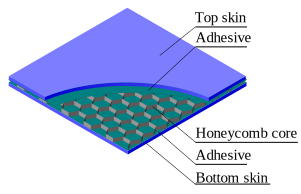
\includegraphics[width=1\linewidth]{../../../figures/png/honeycomb.png}
	\end{center}
	\caption{Sample configuration: a) top view of the sample, b) honeycomb sandwich substructures, c) detail of the honeycomb cell, d) nodes in the spectral element}
	\label{fig:honeycomb}
\end{figure}

\subsection{Simulation parameters}
\label{sec:simulation}
The meshes take into account the damage which was modelled at the bottom skin 
and PZTs attached to the top skin.
The meshes were generated by using external GMSH software 
\cite{geuzaine2009gmsh}.
The meshes were composed of $6 \times 6$ nodes elements.
The mesh density has been chosen to ensure at least 6 nodes per wavelength.
In case of the honeycomb core, one $6 \times 6$ spectral element was used for 
each wall of the cell.

The analysis was made with 15 kHz frequency sine pulse modulated by the Hann 
window.
Total calculation time was set to 800 $\mu$s with time increment $\Delta t=8$ 
ns.
Within this period full pulse of $A_0$ mode passed through the snesnor \#2.
\subsection{Results}
\label{sec:results}
to be continued...
\begin{figure}
	\begin{center}
		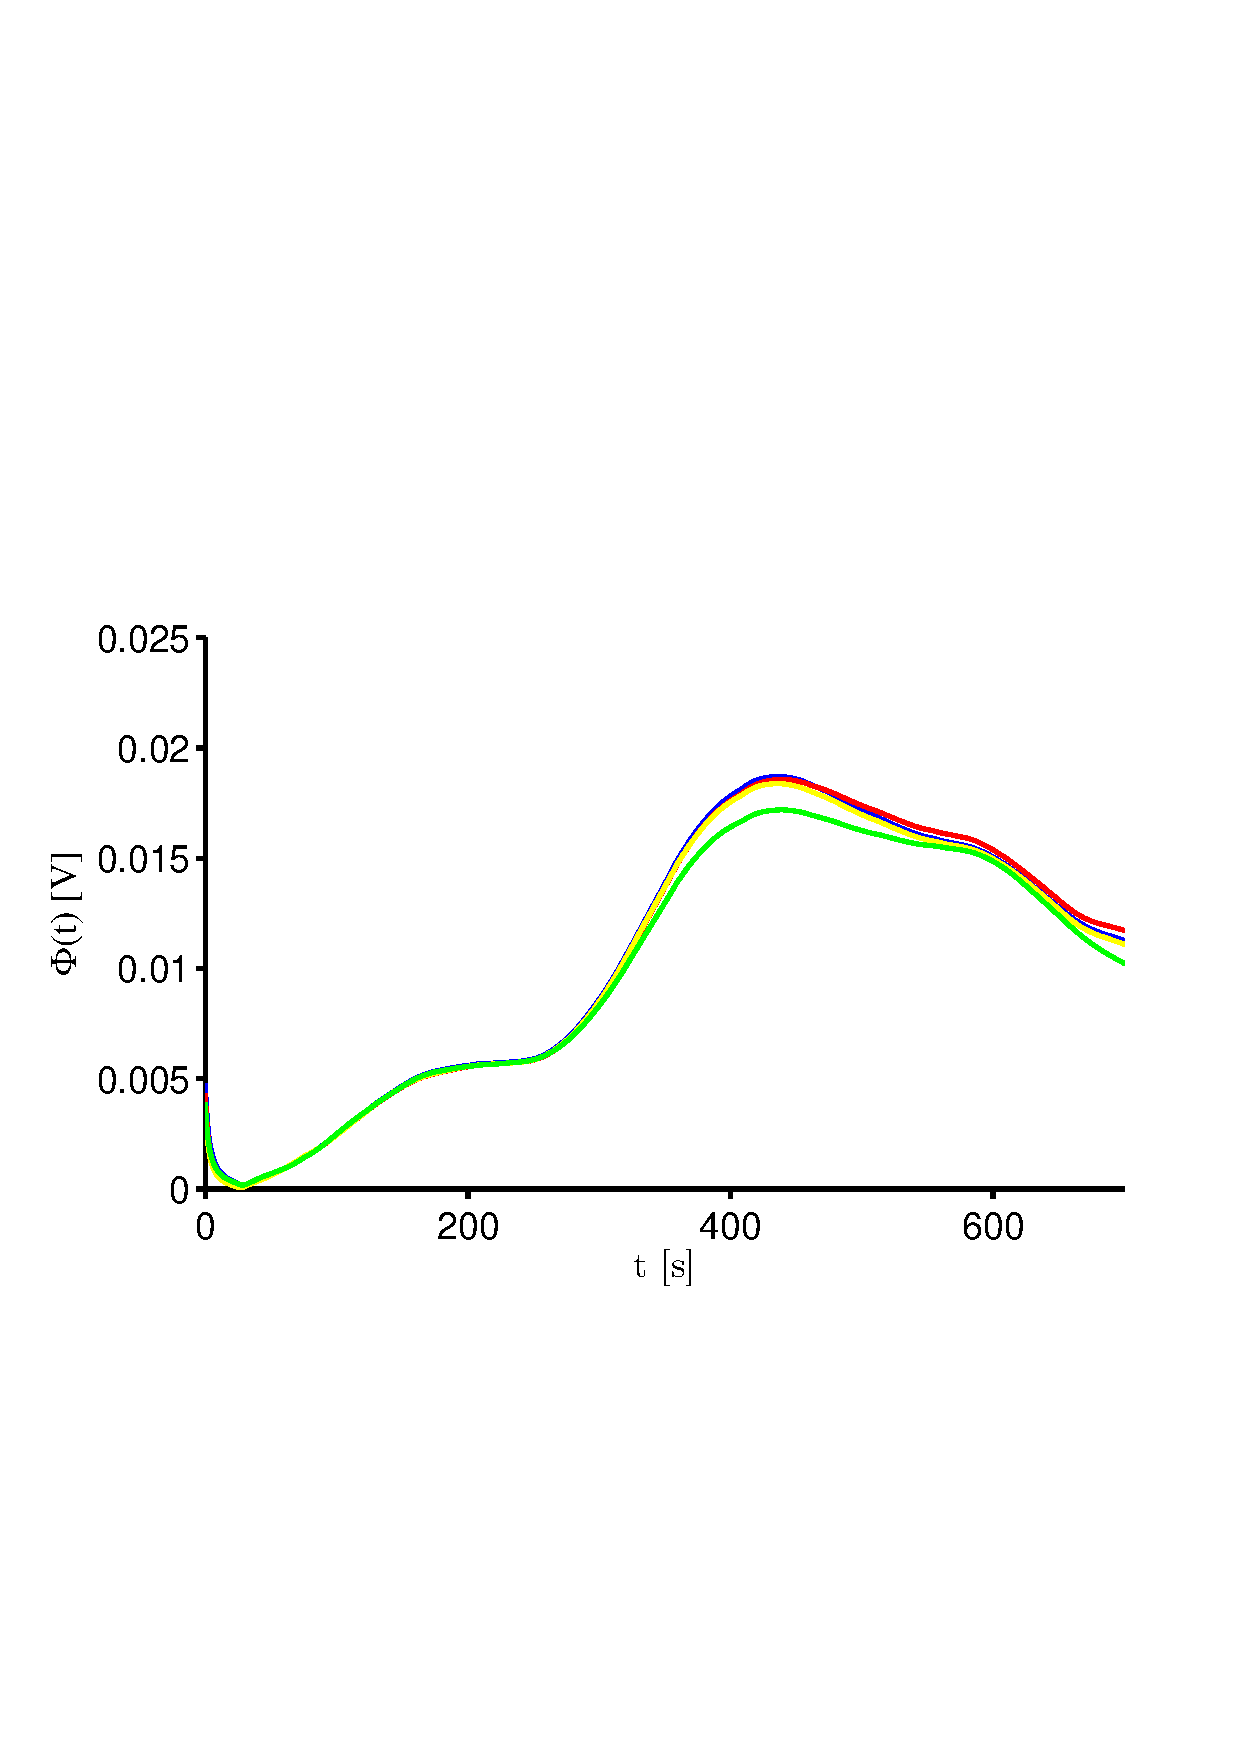
\includegraphics[width=1\linewidth]{../../../figures/png/hilbert.png}
	\end{center}
	\caption{Hilbert}
	\label{fig:hilbert}
\end{figure}
\begin{figure}
	\begin{center}
		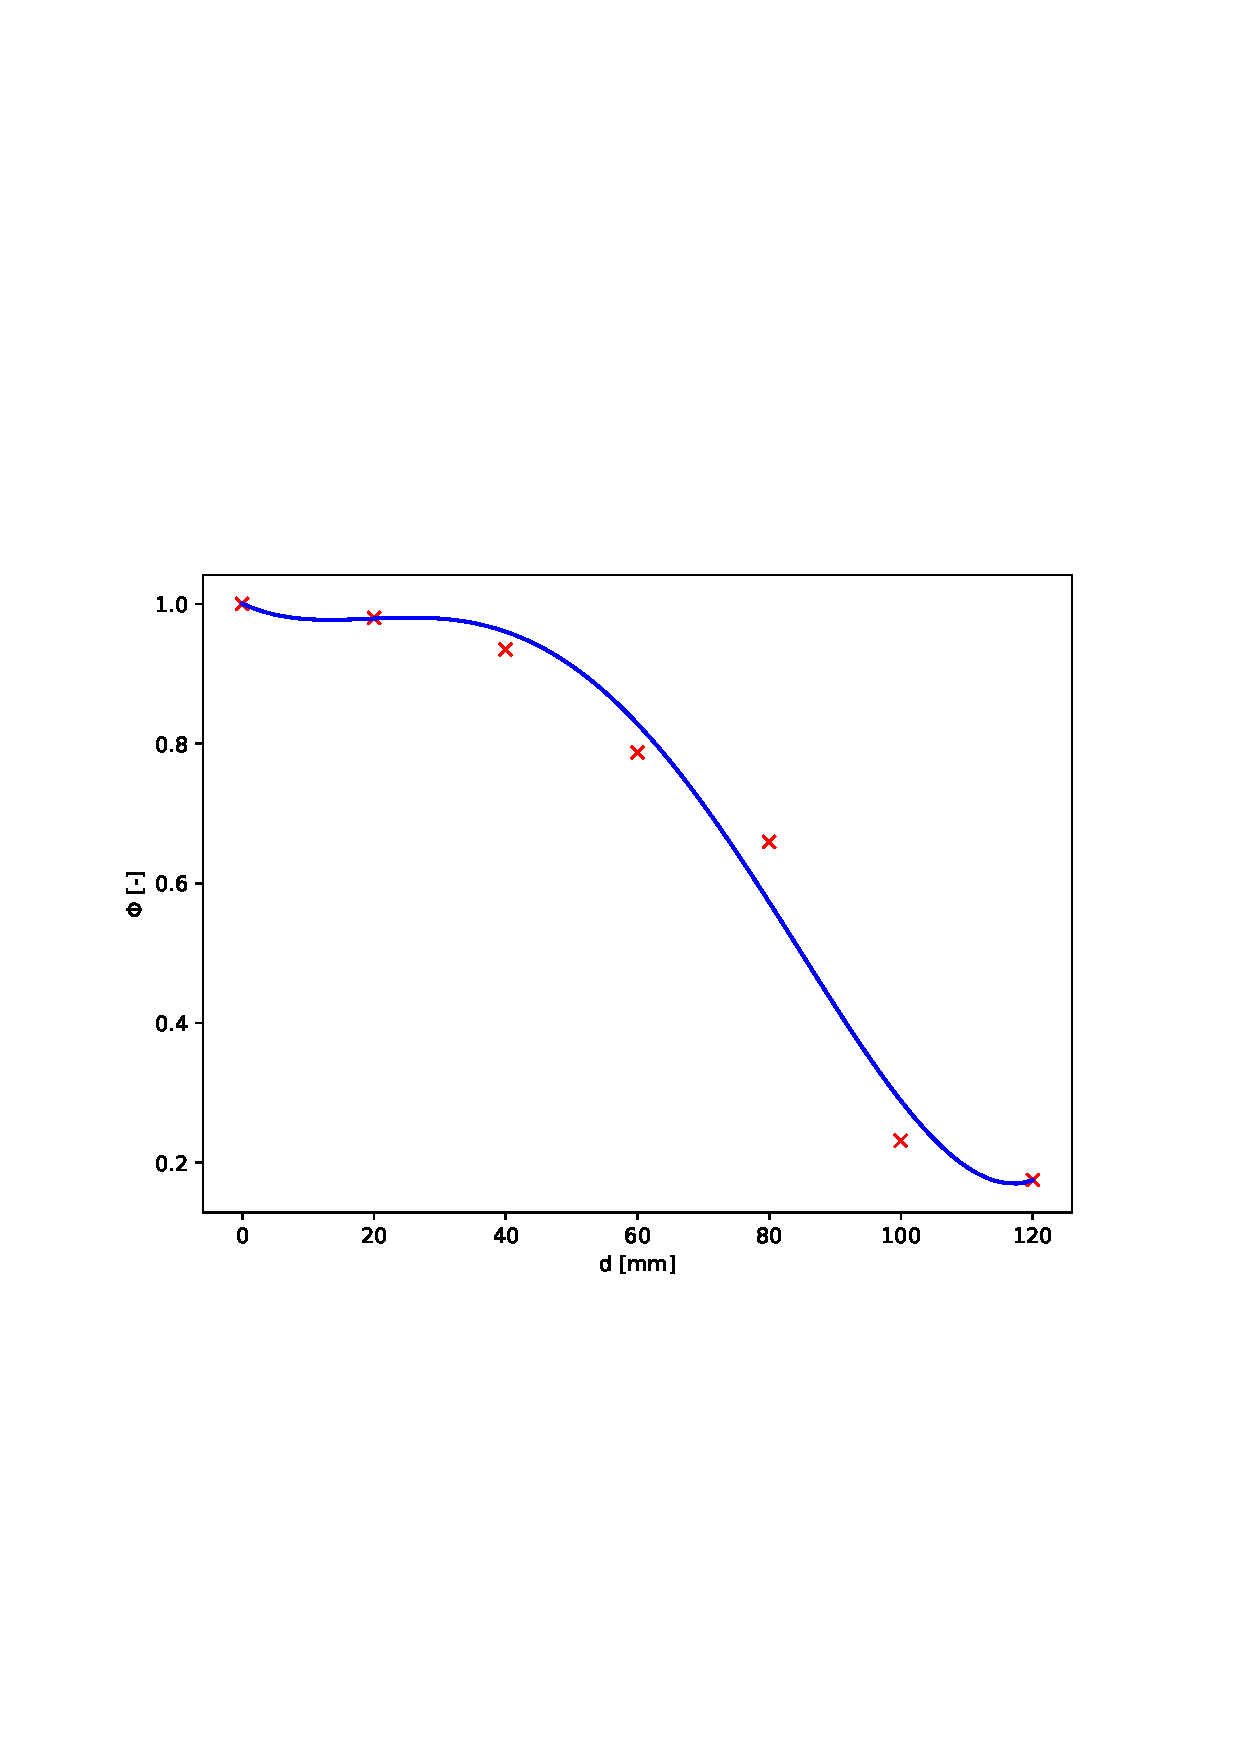
\includegraphics[width=1\linewidth]{../../../figures/png/madif.png}
	\end{center}
	\caption{madif}
	\label{fig:madif}
\end{figure}
\section{Conclusions}
to be continued...
\appendix
\section{}
\label{app:matrices}
The formulae of matrices for 3D elements are:
\begin{eqnarray}
\textbf{M}_{dd}^e & = & \int_{V_e}\textbf{N}^T\rho \textbf{N}\rmd V_e\\
\textbf{K}_{dd}^e & = & \int_{V_e}{\textbf{B}_d^e}^T\textbf{c}\textbf{B}_d^e\rmd V_e
\end{eqnarray}
where \textbf{c} and $\rho$ is the elasticity matrix and mass density, respectively and $\int_{V_e}dV_e$ is a volume integral.

The formulae of matrices for 2D elements are:
\begin{eqnarray}
\textbf{M}_{dd}^e & = & \int_{\Omega_e}\textbf{N}^T\rho 
\left [
\begin{array}{ccccc}
h & 0 & 0 & 0 & 0\\
0 & h & 0 & 0 & 0\\
0 & 0 & h & 0 & 0\\
0 & 0 & 0 & \frac{h^3}{12} & 0\\
0 & 0 & 0 & 0 & \frac{h^3}{12} 
\end{array} \right]
\textbf{N}\rmd \Omega_e\\
\textbf{K}_{dd}^e & = & \int_{\Omega_e}{\textbf{B}_b^e}^T
\left[
\begin{array}{cc}
\textbf{A} & \textbf{B}\\
\textbf{B} & \textbf{D}
\end{array} \right]
\textbf{B}_b^e\rmd \Omega_e+\int_{\Omega_e}{\textbf{B}_s^e}^T\textbf{A}^{\ast}\textbf{B}_s^e\rmd \Omega_e
\end{eqnarray}
where h is the element thickness and $\int_{\Omega_e}d\Omega_e$ is a surface integral and:
\begin{eqnarray}
\textbf{A} & = & \textbf{c}_{ij}(h_t-h_b)\qquad i,j=1,2,6\nonumber\\
\textbf{B} & = & \frac{1}{2}\textbf{c}_{ij}(h_t^2-h_b^2)\qquad i,j=1,2,6\nonumber\\
\textbf{D} & = & \frac{1}{3}\textbf{c}_{ij}(h_t^3-h_b^3)\qquad i,j=1,2,6\nonumber\\
\textbf{A}^{\ast} & = & \kappa \, \textbf{c}_{ij}\left[h_a-4/3\left(h_t^3-h_b^3\right)/h_a^2\right]\qquad i,j=4,5\nonumber
\end{eqnarray}
where the $h_t$ and $h_b$ are the distance from mid-plane to the top and bottom 
layer of the element, respectively and the $\kappa=5/4$ is a shear correction 
factor.

The dielectric conductivity matrix $\textbf{K}_{\phi \phi}^e$ and piezoelectric coupling matrix $\textbf{K}_{u \phi}^e$ are defined:
\begin{eqnarray}
\textbf{K}_{d\phi}^e & = & \int_{V_e}{\textbf{B}_d^e}^T\textbf{e}^T \textbf{B}_{\phi}^e\rmd V_e\\
\textbf{K}_{\phi \phi}^e & = & -\int_{V_e}{\textbf{B}_{\phi}^e}^T {\textbf{$\bepsilon$}^S}^T \textbf{B}_{\phi}^e\rmd V_e
\end{eqnarray}


\section{}
\label{app:properties}

Mechanical properties of carbon fibres, epoxy resin and adhesive layer are 
presented in table~\ref{tab:properties} and evaluated effective elastic 
properties for single layer in table~\ref{tab:properties_layer}.
\begin{table}
\centering
\caption{\label{tab:properties}Material properties of carbon fibres, epoxy resin and adhesive layer}
\begin{tabular}{ccccc}\hline
Material & $E_{11}$ &  $E_{33}$ & $\nu_{12}$ & $\rho$ \\
 & [GPa] &  [GPa] & [-] & [kg/m$^3$]\\
\hline
Carbon & 275.6 & 27.6 & 0.2 & 1900\\
Epoxy & 3.43 & 3.43 & 0.35 & 1250\\
Adhesive & 1.7 & 1.7 & 0.34 & 1200\\
\end{tabular}
\end{table}

\begin{table}
\centering
\caption{\label{tab:properties_layer}Effective material properties of single layer}
\begin{tabular}{cccccccc}
\hline
 $E_{11}$ & $E_{22}$ & $E_{33}$ & $G_{12}$ & $G_{23}$ & $\nu_{12}$ & $\nu_{23}$ & $\rho$ \\
$[$GPa] & [GPa] & [GPa] & [GPa] & [GPa] & [-] & [-] & $[kg/m^3$]\\
\hline
137 & 8.7 & 8.7 & 3.61 & 3.19 & 0.28 & 0.37 & 1569\\
\hline
\end{tabular}
\end{table}


Material properties of the PZT transducer:
\begin{eqnarray}
\textbf{c}^E=\left [ 
\begin{array}{cccccc}
134 & 88.9 & 90.9 & 0 & 0 & 0 \\ 
88.9 & 134 & 90.9 & 0 & 0 & 0 \\
90.9 & 90.9 & 121 & 0 & 0 & 0 \\
0 & 0 & 0 & 20.5 & 0 & 0 \\
0 & 0 & 0 & 0 & 20.5 & 0 \\
0 & 0 & 0 & 0 & 0 & 22.4 \nonumber \\
\end{array}
\right ] \left [ GPa \right ] 
\end{eqnarray}
\begin{eqnarray}
\textbf{e}=\left[
\begin{array}{cccccc}
0 & 0 & 0 & 0 & 13.7 & 0\\
0 & 0 & 0 & 13.7 & 0 & 0\\
-6.06 & -6.06 & 17.2 & 0 & 0 & 0\nonumber \\
\end{array}
\right] \left[C\ m^{-2}\right]
\end{eqnarray}
\begin{eqnarray}
\bepsilon^S_r=\left[
\begin{array}{ccc}
906 & 0 & 0\\
0 & 906 & 0\\
0 & 0 & 823\nonumber \\
\end{array}
\right] \left[ - \right]
\end{eqnarray}
\begin{eqnarray}
\rho=7850\ [kg\ m^{-3}] \nonumber
\end{eqnarray}

\bibliography{../../../../../BibTex/Rozprawa}{}
\end{document}